\section{Durchführung}
\label{sec:Durchführung}
Die Messapparatur vor Ort ist nach dem Schema in \autoref{fig:aufbauschema} aufgebaut worden.
\begin{figure}
    \centering
    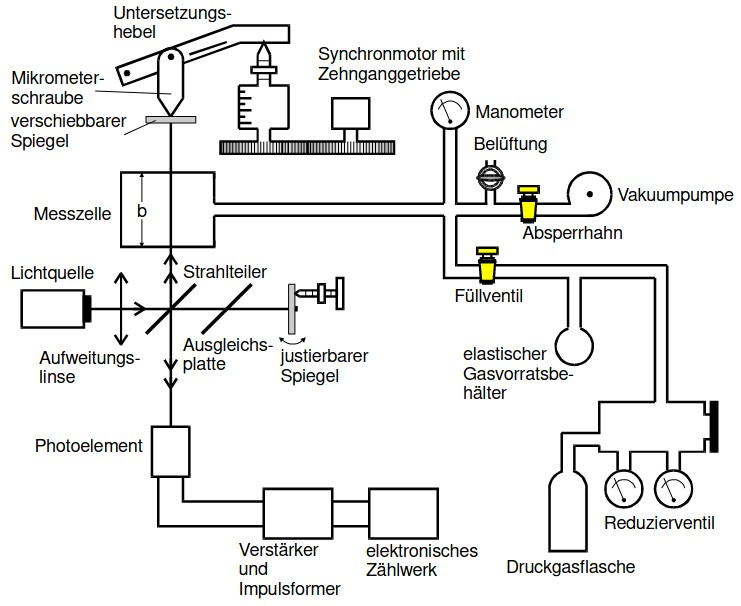
\includegraphics[width=\textwidth]{content/aufbauversuch.jpg}
    \caption{Der schematische Aufbau der Messapparatur vor Ort.}
    \label{fig:aufbauschema}
\end{figure}

\noindent
Nachdem der Raum vollständig abgedunkelt wurde, damit keine Änderung der Lichtverhältnisse das Messergebnis verfälschen kann, wurde das Interferometer einjustiert.
Dafür wurde vor den Detektor eine Mattscheibe gehalten und die am hellsten zu sehenden Punkte wurden zur Deckung gebracht. Außerdem wurde die als Detektor benutzte
Photozelle so ausgerichtet, dass das Interferenzbild genau auf den Eintrittsspalt fällt.


\subsection{Bestimmung der Wellenlänge des Lasers}
Nun kann die Messung zur Bestimmung der Wellenlänge von Laser begonnen werden. Dafür wird von einem Motor mit Hilfe einer Mikrometerschraube der verschiebbare 
Spiegel jeweils um $\SI{5}{\milli\meter}$ verschoben und die in diesem Vorgang durchlaufenden Maxima gezählt. Das Zählen der durchlaufenden Maxima wird von der 
Photozelle übernommen. Es ist wichtig, darauf zu achten, dass der Spiegel nicht zu schnell verschoben wird, da sonst manche Maxima nicht detektiert werden können.
Es wurde darauf geachtet, dass die Mikrometerschraube auf 0 steht, dann vom Motor bis $\SI{5}{\milli\metre}$ aufgedreht wird. Die bei dieser Bewegung durchlaufende
Maximaanzahl wurde notiert. Dann hat der Motor die Schraube etwas weiter aufgedreht. Anschließend wurde der Spiegel wieder um ca $\SI{5}{\milli\meter}$ bewegt und 
die Maximaanzahl notiert, wobei jetzt der Spiegel in die andere Richtung bewegt worden ist. Dieser Messvorgang wird fünf mal wiederholt.


\subsection{Bestimmung des Brechungsindexes von Luft}
Zu Bestimmung der Brechungsindexes wird der Aufbau des Experimentes nicht verändert. In der einen Strecke befindet sich eine Messzelle, welche mit Luft gefüllt ist.
Nun wird die Anzahl der durchlaufenden Maxima gezählt, während bis zu einer gewissen Druckanzahl mit einer Vakuumpumpe die Luft aus der Messzelle gepumpt wird.
Dann wird langsam die Luft wieder in die Messzelle gelassen; hierbei wird auch nochmal die Maximaanzahl notiert. Es ist hier sehr wichtig, schnell den Wert zu notieren,
wenn der Druck erreicht ist und die Luft einströmen zu lassen, weil dieser Druck von der Messapparatur nicht lange gehalten wird. Der Messvorgang wird einige Male 
wiederholt.

\begin{figure}
    \centering
    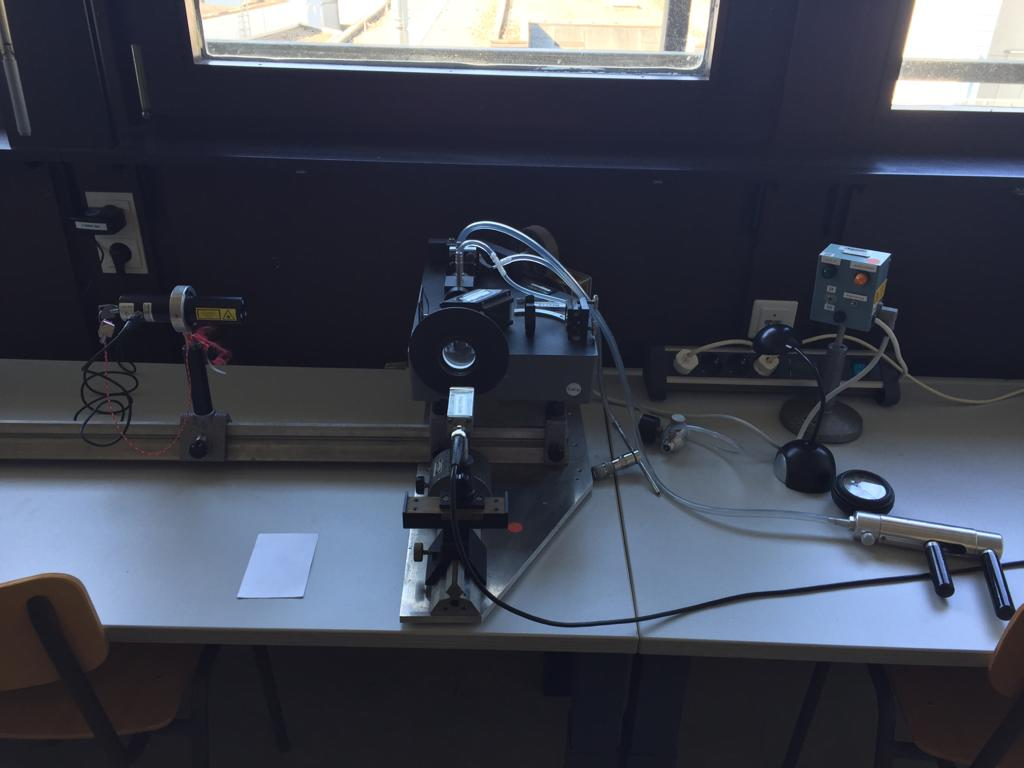
\includegraphics[width=0.6\textwidth]{content/aufbaufoto1.jpeg}
    \caption{Der Versuchsaufbau vor Ort. Links ist der Laser zu sehen, welcher auf den semipermeablen Spiegel gerichtet ist. Hinter den Schläuchen ist der verstellbare
    Spiegel und der Motor zu erkennen. Der Spiegel rechts auf der Apparatur hat die Schrauben zum Justieren. Vor der Apparatur ist die Zestrungslinse und der Detektor.
    Der bläuliche Kasten beinhaltet die Schalter für den Motor und die Schläuche verbinden die Messzelle auf der Apparatur mit dr Vakuumpumpe auf dem Tisch.}
\end{figure}

\begin{figure}
    \centering
    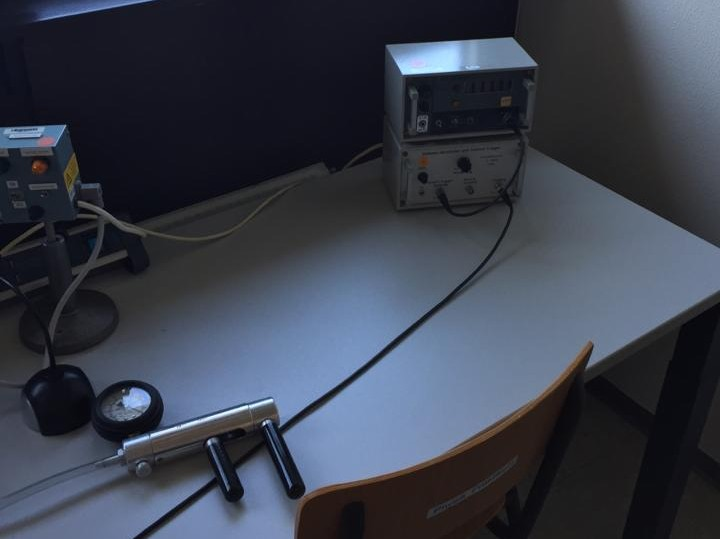
\includegraphics[width=0.6\textwidth]{content/aufbaufoto2.jpeg}
    \caption{Hier ist der Impulszähler auf dem Selektivverstärker zu sehen.}
\end{figure}